\section{Arquitectura base (modelo C4)}

Describimos el sistema con los dos primeros niveles del modelo C4: el diagrama de contexto (nivel~1) y el de contenedores (nivel~2). Los dos se hicieron en draw.io, y los archivos editables y sus exportaciones están en \nolinkurl{docs/diagramas/}. En los diagramas y en este documento el sistema se llama \emph{Sistema de gestión de pre-sustentaciones}.

\subsection{Del primer bosquejo al diagrama C4}

La arquitectura empezó como un bosquejo a mano del 20 de noviembre de 2026 (figura~\ref{fig:bosquejo}). Ese bosquejo ya tenía los cinco actores, la aplicación web, el API Gateway, los cinco servicios, cuatro bases de datos, el almacenamiento de los PDF y la cola de mensajes. Al pasarlo a C4 hicimos cinco cambios:

\begin{itemize}
  \item agregamos la tecnología de cada contenedor y el protocolo de cada flecha;
  \item agregamos los sistemas externos del nivel~1: URKUND, el servicio de correo y el SGA;
  \item agregamos una llamada directa de Evaluación y actas a Solicitudes y documentos, porque antes de abrir la rúbrica hace falta saber si el informe y el reporte de URKUND ya están;
  \item le dimos a Notificaciones su propia base, para guardar los avisos enviados y los que faltan por enviar;
  \item guardamos el porcentaje de URKUND como un dato de la base de Solicitudes, y no solo dentro del PDF.
\end{itemize}

\begin{figure}[htbp]
  \centering
  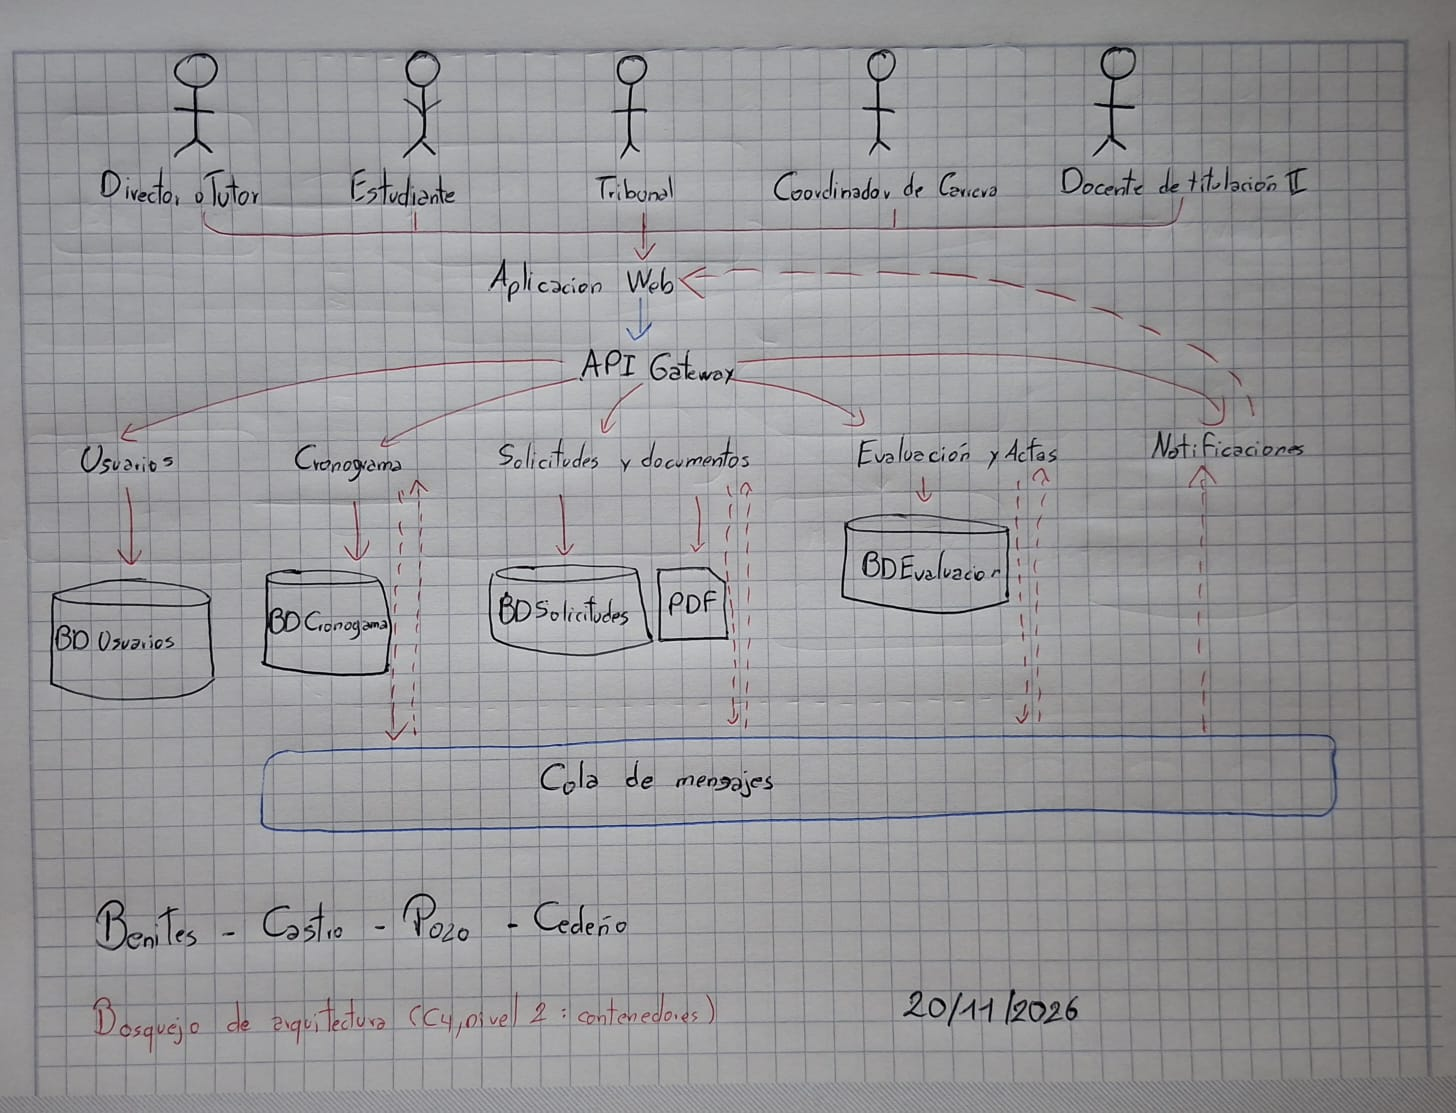
\includegraphics[width=0.68\textwidth]{../evidencias/fotos/primer-bosquejo-arquitectura-2026-11-20.jpeg}
  \caption{Primer bosquejo de la arquitectura, hecho a mano el 20 de noviembre de 2026.}
  \label{fig:bosquejo}
\end{figure}

\subsection{Nivel 1: contexto}

La figura~\ref{fig:c4-n1} muestra el sistema como una caja cerrada, con quienes lo usan y con los sistemas que están alrededor. Los cinco actores salen de la entrevista:

\begin{itemize}
  \item el estudiante sube su informe y el reporte de URKUND, y sigue su trámite;
  \item el director o tutor revisa el porcentaje de coincidencia en URKUND, lo registra en el sistema y sube sus informes;
  \item el tribunal, formado por un presidente y dos miembros, califica la predefensa con la rúbrica;
  \item el coordinador de carrera arma el cronograma;
  \item el docente de Titulación~II pone su 60~\% de la nota y consolida la nota final.
\end{itemize}

El sistema solo se comunica con el servicio de correo, por SMTP, para enviar los avisos. Con URKUND y con el SGA no se conecta: el director usa URKUND por fuera, y el docente de Titulación~II registra la nota final en el SGA a mano, como se hace hoy. La aprobación del anteproyecto queda fuera del alcance porque es una etapa previa. La secretaría tampoco aparece, porque se encarga del acta de la sustentación final y no de la predefensa.

\begin{figure}[htbp]
  \centering
  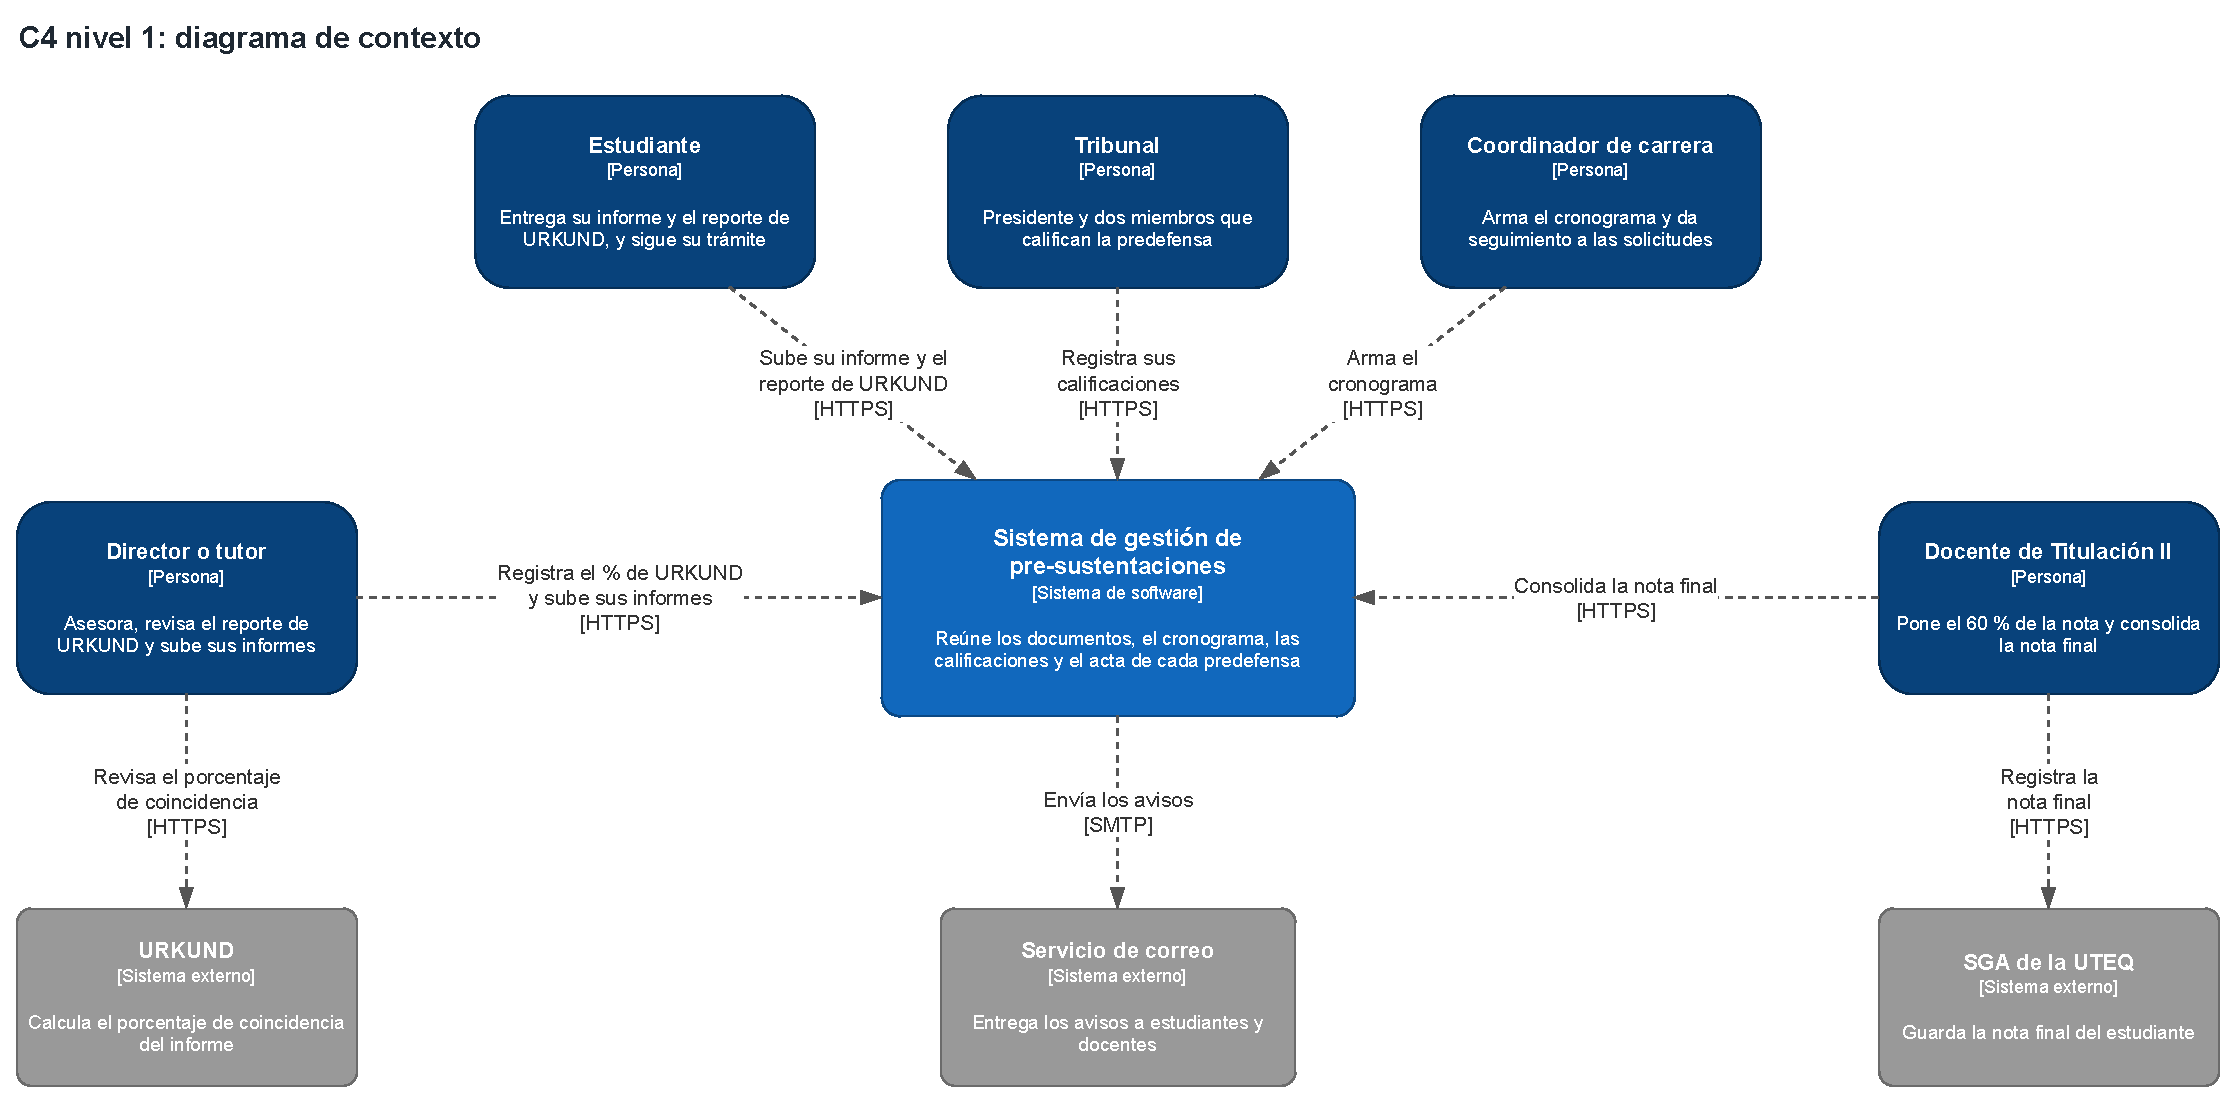
\includegraphics[width=\textwidth]{c4-nivel1-contexto.pdf}
  \caption{C4 nivel 1: diagrama de contexto.}
  \label{fig:c4-n1}
\end{figure}

\subsection{Nivel 2: contenedores}

La figura~\ref{fig:c4-n2} abre la caja del sistema. Los usuarios entran desde el navegador a la aplicación web, que manda cada petición al API Gateway con el JWT de la sesión. El gateway valida el JWT y envía la petición al servicio que corresponde. La tabla~\ref{tab:contenedores} resume cada contenedor.

\begin{figure}[htbp]
  \centering
  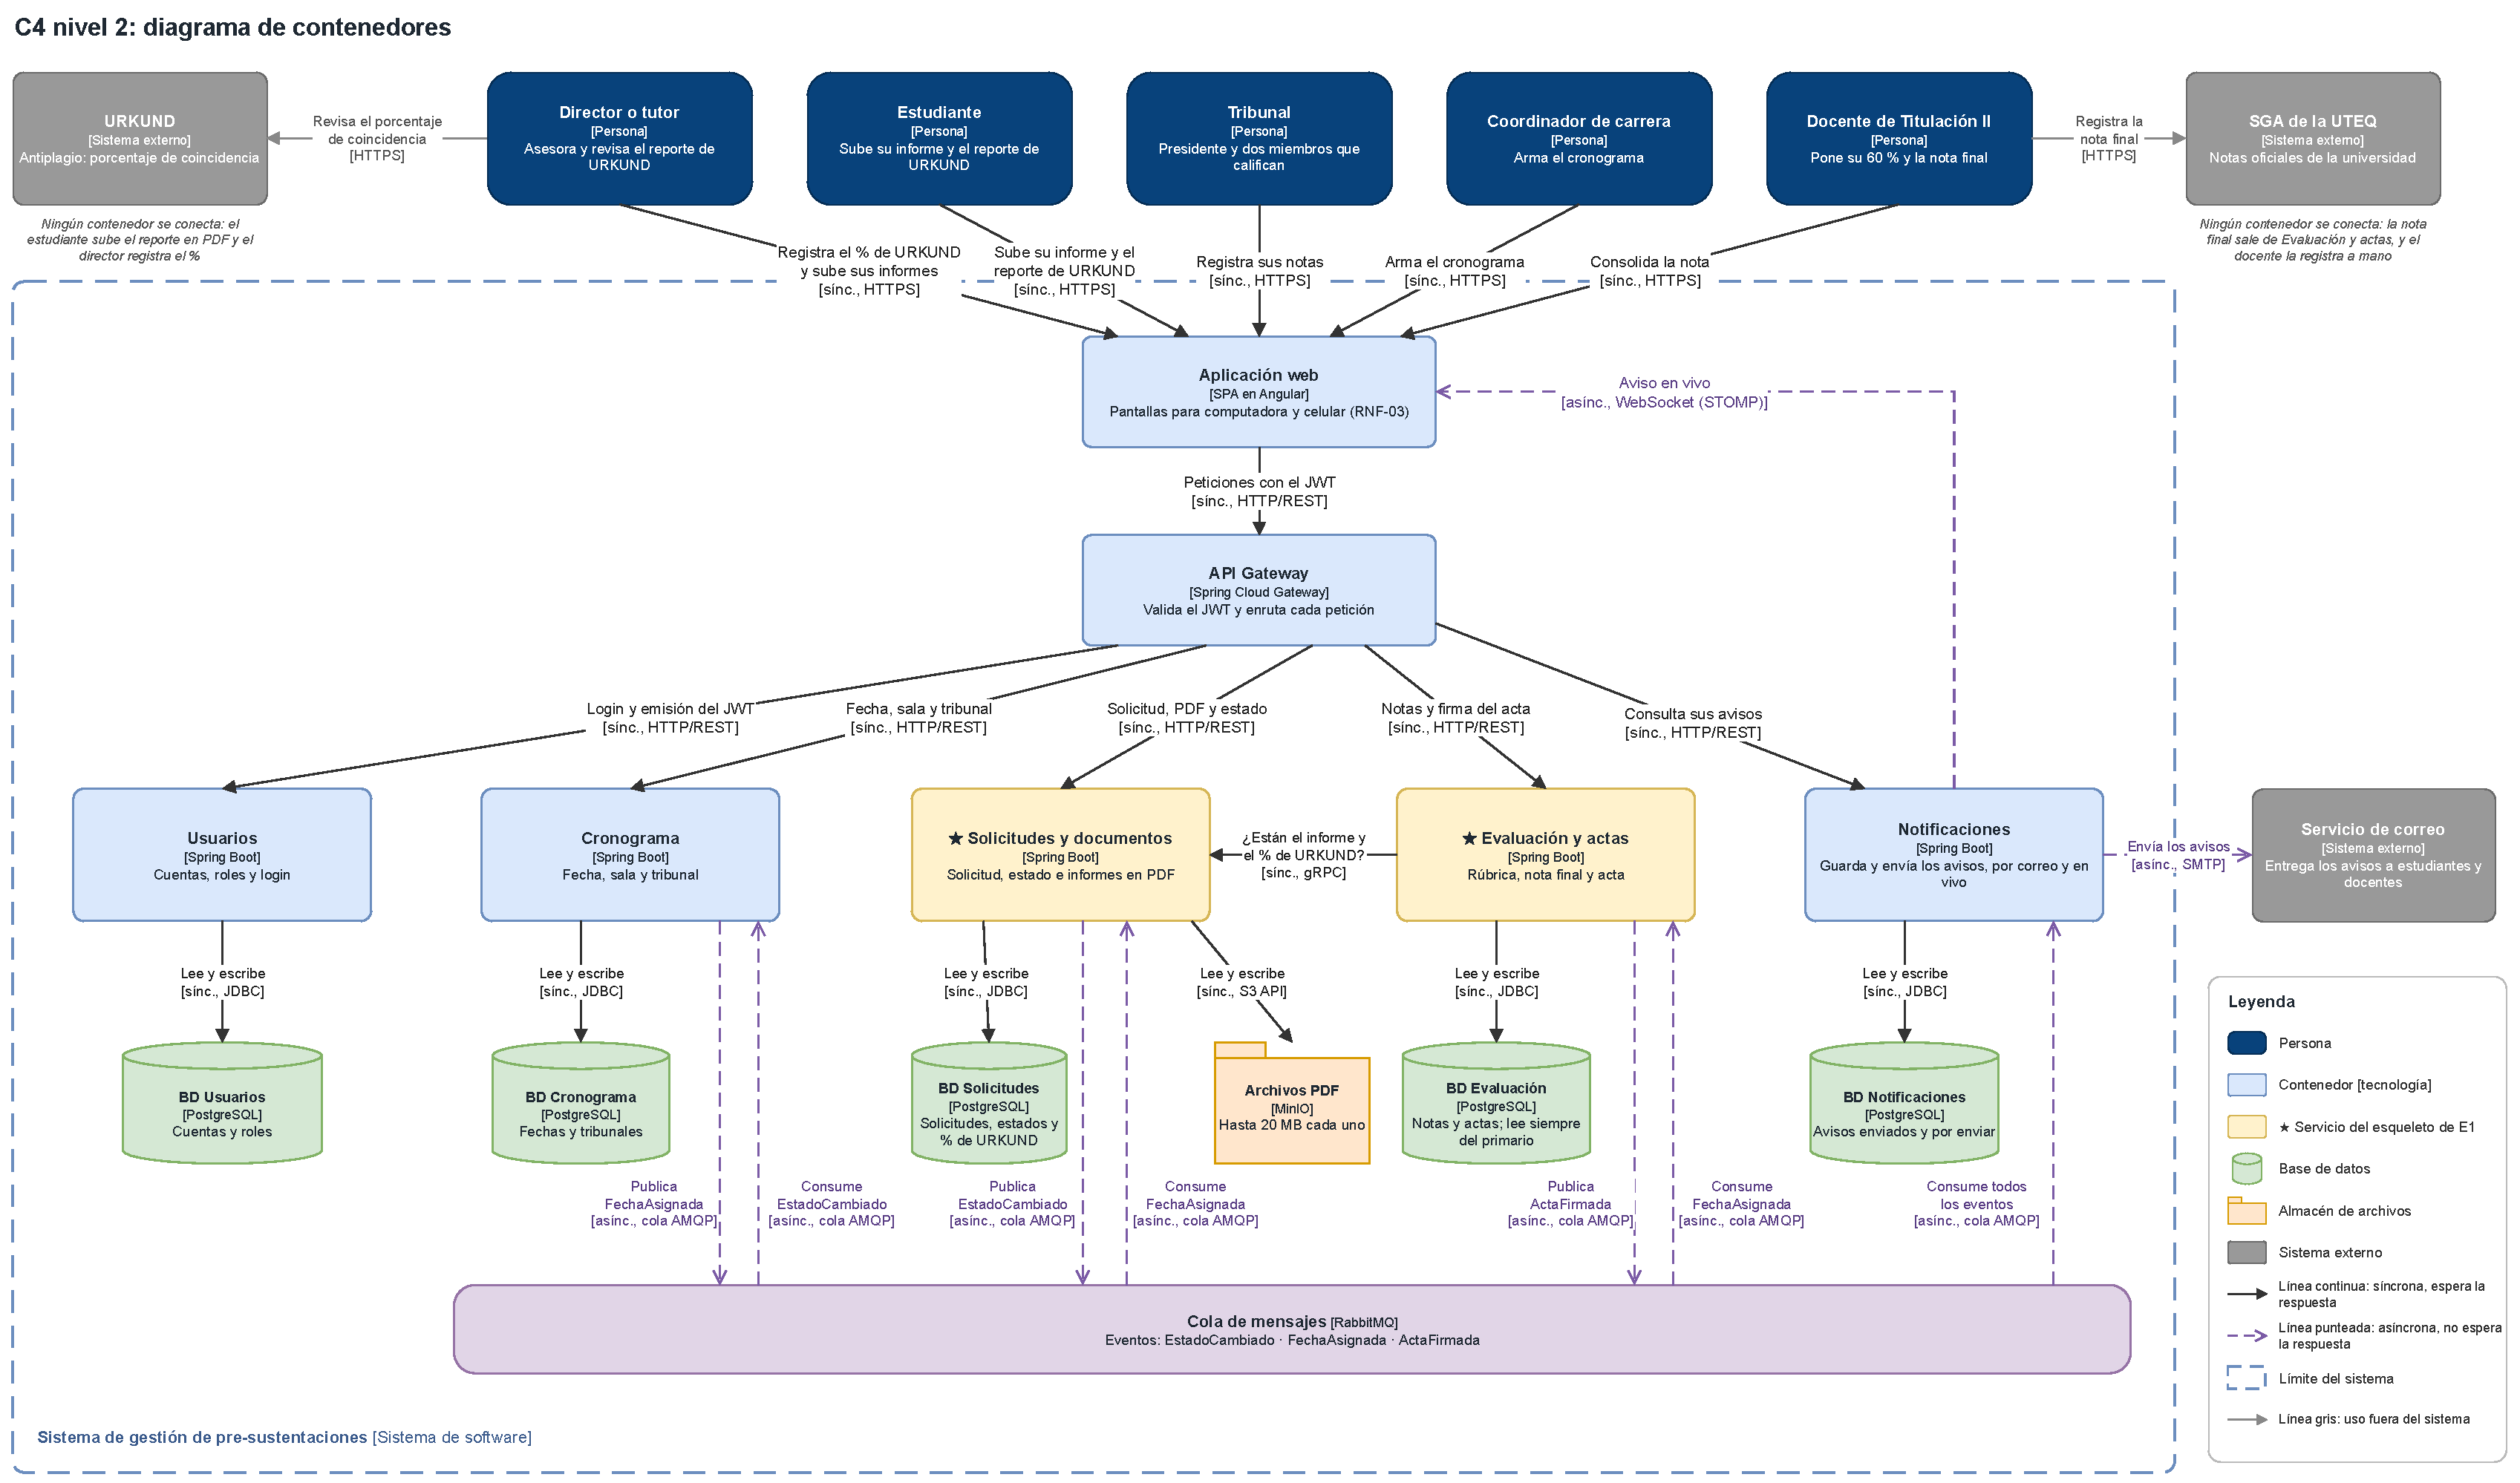
\includegraphics[width=\textwidth]{c4-nivel2-contenedores.pdf}
  \caption{C4 nivel 2: diagrama de contenedores. Las líneas continuas son llamadas síncronas y las punteadas, asíncronas.}
  \label{fig:c4-n2}
\end{figure}

\begin{table}[htbp]
  \centering
  \caption{Contenedores del sistema.}
  \label{tab:contenedores}
  \small
  \begin{tabularx}{\textwidth}{@{}>{\raggedright\arraybackslash}p{2.9cm} >{\raggedright\arraybackslash}p{2.6cm} >{\raggedright\arraybackslash}X >{\raggedright\arraybackslash}p{2.6cm}@{}}
    \toprule
    \textbf{Contenedor} & \textbf{Tecnología} & \textbf{Qué hace} & \textbf{Datos} \\
    \midrule
    Aplicación web & Angular & Pantallas para computadora y celular (RNF-03) & --- \\
    API Gateway & Spring Cloud Gateway & Única entrada: valida el JWT y enruta cada petición & --- \\
    Usuarios & Spring Boot & Cuentas, roles, inicio de sesión y emisión del JWT & BD Usuarios \\
    Cronograma & Spring Boot & Fecha, sala y tribunal de cada predefensa & BD Cronograma \\
    Solicitudes y documentos & Spring Boot & Solicitud, estado, informes en PDF y porcentaje de URKUND & BD Solicitudes y MinIO \\
    Evaluación y actas & Spring Boot & Rúbrica, nota final (40~\% del tribunal y 60~\% del docente) y acta & BD Evaluación \\
    Notificaciones & Spring Boot & Avisos por correo y en vivo & BD Notificaciones \\
    Cola de mensajes & RabbitMQ & Eventos \texttt{EstadoCambiado}, \texttt{FechaAsignada} y \texttt{ActaFirmada} & --- \\
    \bottomrule
  \end{tabularx}
\end{table}

Las bases de datos usan PostgreSQL. Cada servicio tiene la suya, y ningún servicio lee la base de otro: si necesita un dato, se lo pide al servicio dueño o lo recibe por un evento. Los PDF van en MinIO, fuera de las bases. Solicitudes y documentos y Evaluación y actas, marcados con una estrella en la figura, son los dos servicios del esqueleto de esta entrega (sección~13). El tipo y el mecanismo de cada interacción están en la sección~8, y lo que se prioriza con cada dato crítico, en la sección~9.
